\section{Treniranje SSD neuronske mreže}
\subsection{Visoki pogled na treniranje}
Bitna razlika u treniranju \emph{SSD} mreže i tipične \emph{R-CNN} mreže slične zadaće je ta da "ground truth" podatak mora biti dodjeljen točnom izlazu iz fiksnog skupa izlaza detektora (\cite{liu2016ssd}).
Na sličan način radi i veliko poboljšanje na \emph{R-CNN} arhitekturu, \emph{Faster R-CNN}. \\
Kao i kod klasičnih neuronskih mreža, primjenjuje se funkcija gubitka, a za određivanja težina koristi se \emph{back propagation} od kraja do kraja.
Prije početka treniranja također se određuju pretpostavljeni kvadrati, različite skale za detekciju i strategije za povećanje podataka. \\
O pretpostavljenim kvadratima, skalama za detekciju i strategijama pisati ću u nastavku.
\subsection{Određivanje pozicije objekata}
Tijekom treninga, cilj je odrediti koji pretpostavljeni kvadrati najbolje odgovaraju "ground truth" kvadratima objekta, to jest onima specifiranim u dataset-u.
Nakon što se odrede najprecizniji kvadrati, mreža se sukladno tome dalje prilagođava.
Za svaki "ground truth" kvadrat imamo na izbor više pretpostavljenih kvadrata, različitih lokacija, skala i omjera.
Želimo naći onaj koji ima najveći \emph{jaccardov index preklapanja} (dalje \emph{IoU}) (slika ~\ref{fig:JaccardIndex}).
\begin{figure}[h!]
	\centering
	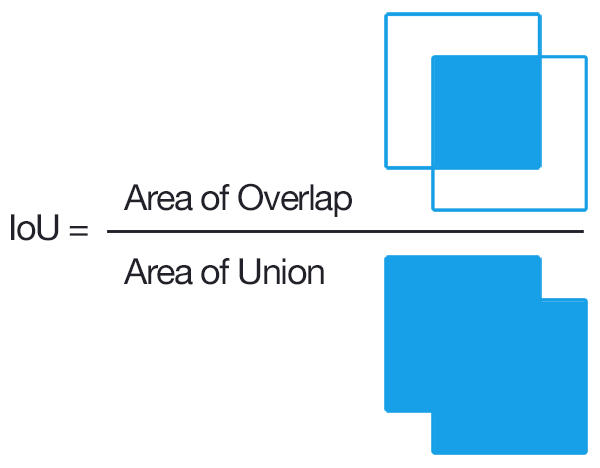
\includegraphics[width=0.6\linewidth]{iou_equation}
	 \caption{Način na koji računamo \emph{jaccardov index preklapanja, tj. IoU}}
 	 \label{fig:JaccardIndex}
\end{figure} \\
U konfiguracijskoj datoteci koja će biti priložena na kraju rada, možemo ručno odrediti od koje točke pretpostavljeni kvadrat prihvačamo.
Pretpostavljena vrijednost je da mora vrijediti $IoU \geq 0.5$.
To višestruko olakšava treniranje jer mreža zadržava više pretpostavljenih kvadrata umjesto da mora odabrati samo onaj sa najvećim preklapanjem.
\subsection{Određivanje parametara za nastavak treniranja}
Određivanje parametara bilo bi puno lakše kada bismo imali samo jedan objekt za klasificirati, no postaje kompliciranije sa više objekata.
Uzmimo $x^p_{ij}=\{1,0\}$ kao indikator za podudaranje $i$-tog pretpostavljenog kvadrata na $j$-ti "ground truth" kvadrat kategorije $p$.
Koristeći spomenutu strategiju određivanja pozicije objekata može nam se dogoditi situacija $\sum_i{x_{ij}^p} \geq 1$. \\
Ukupna funkcija gubitka računa se kao otežana suma lokalizacijskog (\emph{loc}) i klasifikacijskog (\emph{conf}) gubitka:
$$L(x,c,l,g)=\frac{1}{N}(L_{conf}(x,c)+\alpha L_{loc}(x,l,g))$$
$N$ nam predstavlja broj "pogođenih" pretpostavljenih kvadrata. Naravno, ako je $N=0$, postavimo da je gubitak također $=0$.
\subsubsection{Lokalizacijski gubitak (\emph{loc})}
Za izračun lokalizacijskog gubitka koristimo \emph{Smooth L1} između predviđenih i "ground truth" kvadrata.
$$L_{loc}(x,l,g)=\sum_{i\in Pos\ m \in\ (cx, cy, w, h)}^{N} \ \sum x_{ij}^k\ smooth_{L1}(l_i^m - \hat g_j^m)$$
\subsubsection{Klasifikacijski gubitak (\emph{conf})}
Klasifikacijski gubitak računa se kao \emph{softmax} svih klasa koje podržavamo. 
$$L_{conf}(x,c)=-\sum_{i \in Pos}^N x_{ij}^p \log(\hat c_i^0) - \sum_{i \in Neg} \log(\hat c_i^0 ) \ {gdje} \ \hat c_i^p=\frac{\exp(c_i^p)}{\sum_p \exp(c_i^p)}$$
